\documentclass[11pt]{article}
\usepackage[T1]{fontenc}
\usepackage[utf8]{inputenc}
\usepackage{lmodern,amsmath,amssymb,graphicx,geometry,microtype,setspace,booktabs,caption}
\usepackage[hidelinks]{hyperref}
\geometry{letterpaper,margin=1in}
\setlength{\parindent}{0pt}
\setlength{\parskip}{0.55em}
\setlength{\emergencystretch}{2em}
\captionsetup{labelfont=bf,font=small}
\renewcommand{\refname}{References}
\pagestyle{empty}
\renewcommand{\thefigure}{S\arabic{figure}}
\setcounter{figure}{0}
\begin{document}
\begin{figure}[!ht]\centering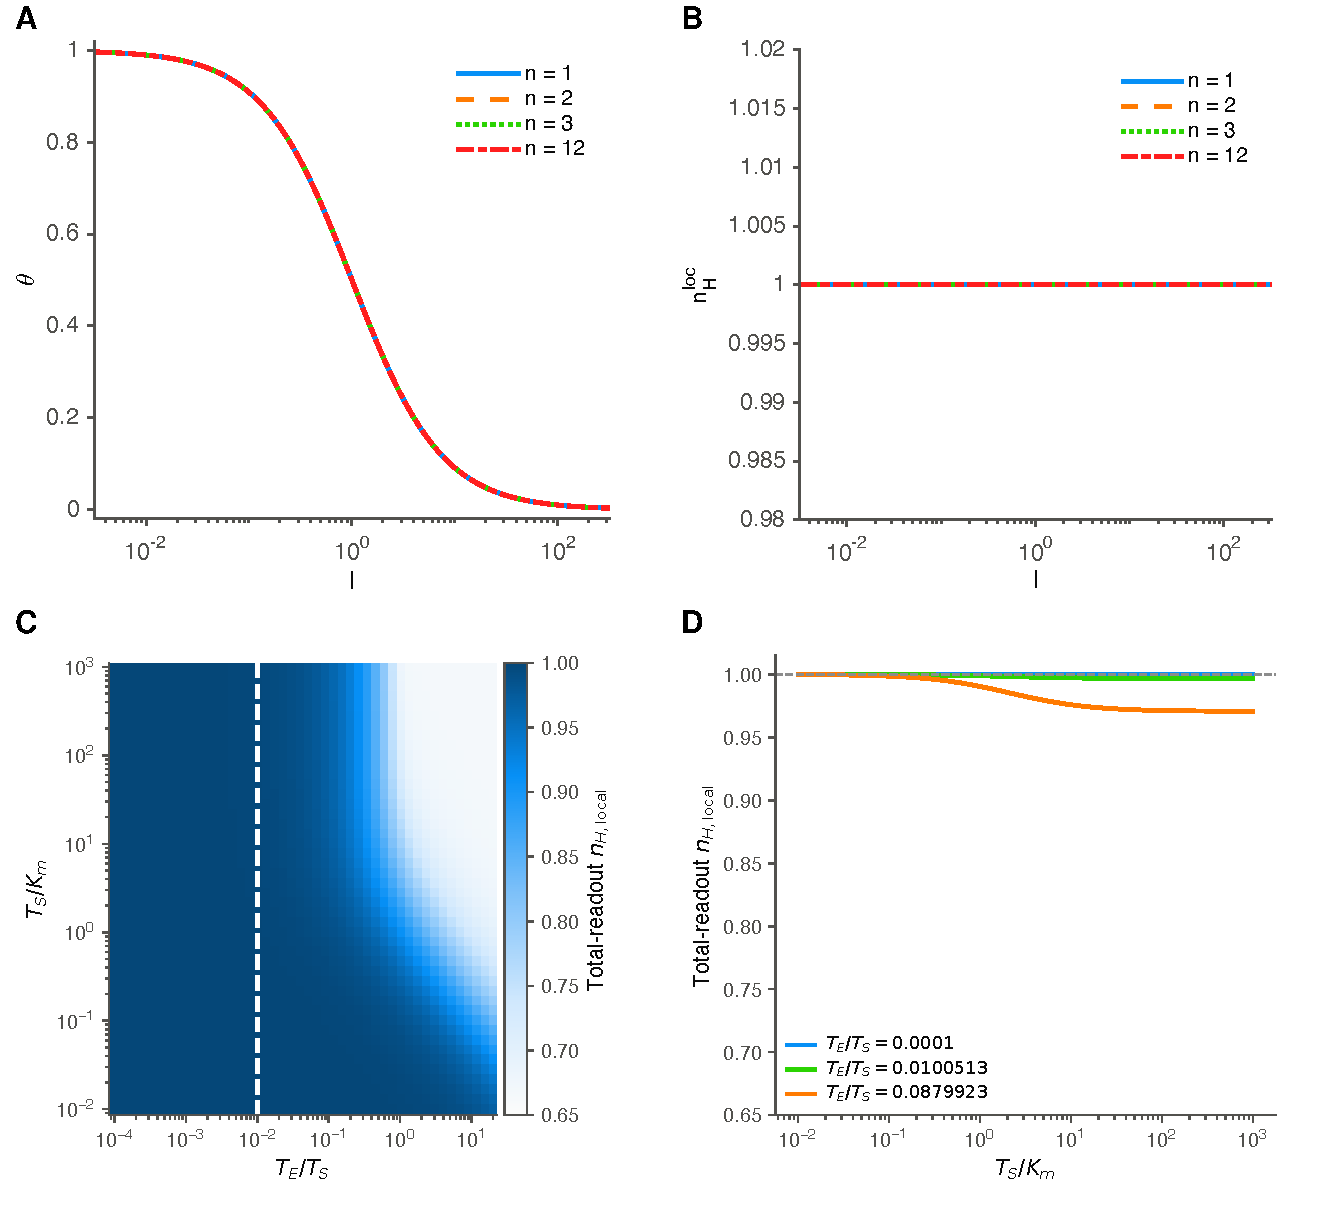
\includegraphics[width=\textwidth,height=0.60\textheight,keepaspectratio]{figure_inputs/FigS11_extended.pdf}\caption{\textbf{Independent-site invariance and the experimentally accessible readout.} (A) Free-target mean modified fractions for n=1, 2, 3, and 12 identical independent sites coincide, with dimensionless input and unit midpoint. (B) Their local coefficients equal one throughout. (C) Local coefficient of the total-target readout at half-response across enzyme-to-target ratio and target saturation in the specified three-site model; the dashed line marks $T_E$/$T_S$=0.01. (D) Representative slices. For $T_E$/$T_S$ at most 0.01 the coefficient remains at least 0.99745 across the plotted saturation range. Panels C and D are numerical calculations for the stated model; the exact invariant in A and B concerns free target.}


\end{figure}
\end{document}
